\documentclass{article}
\usepackage{Preamble}


\title{Problem 1: Factorial  \\[8pt] CS3305 Data Structures}
\author{Casey Hampson}

\begin{document}
\maketitle


\section*{Algorithm Description}
This bit was listed in the assignment description but not in the deliverable section, but I'll include it anyway. Since this one is so simple, I'll just use plain words to describe this rather than pseudo-code or something.

We will have a function called \mintinline{java}{Factorial} which takes in the user input that we want to compute the factorial of. We then establish the base case, which is whenever the number reaches 1 (or less, just in case); in such a case, we want to just return the number itself, i.e. 1. From there, the definition of factorial is $n! = n(n-1)(n-2)...$, so we want to return the current number multiplied by the function itself with an input of one less than the current input. This will continue chaining back until it reaches the base case, 1, so we end up computing the factorial.



\section*{Program Output}

    \begin{figure}[htbp]
        \centering
        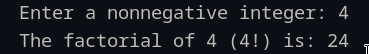
\includegraphics[scale=0.75]{res/4.png}
        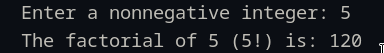
\includegraphics[scale=0.75]{res/5.png}
        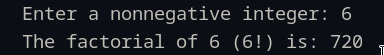
\includegraphics[scale=0.75]{res/6.png}
    \end{figure}

\pagebreak
\section*{Source Code}
\inputminted{java}{./P1.java}


\end{document}
